% vim:ft=tex
% rubber: module xelatex

\subsection{Distortion removal}
\label{sec:distortion}

We investigated forms of distortion removal independent of camera calibration. An open-source ANSI C library for this is provided by the authors of \cite{algebraic-distortion}. Herein we shall refer to this unnamed library and the algorithm it describes as IPOLdistortion. This implementation estimates the lens distortion parameters in terms of coefficients $\kappa_{0}$, $\kappa_{2}$, and $\kappa_{4}$, and provides a correction function. See section~\ref{sec:distortion-prior} for discussion of the IPOLdistortion method.

\subsubsection{Implementation notes}

The IPOLdistortion library requires that users manually select points on the straight line for the algorithm to work on. This can be an arduous process for the user, and is susceptible to human error. Furthermore, \cite{algebraic-distortion} state that for the maximum efficacy, as many straight lines as possible should be used. Therefore in our implementation, we combine the distortion correcting functionality of IPOLdistortion with the autonomous line extraction functionality of OpenCV. 

We use OpenCV to automatically extract detected corner points from a (distorted) chessboard image. From these corner points, and our knowledge of the chessboard dimensionality (number of squares per side), we can reconstruct segments which ``should" be straight lines in the image. The algorithm we use for this is relatively naive, relying on the fact that OpenCV returns corners in a fixed order. The algorithm is likely to fail if this list is out of order for some reason. To secure high-quality performance, we provide the algorithm with all the horizontal line segments and two vertical line segments returned by the OpenCV code.

The actual distortion removal functionality provided by IPOLdistortion consists of first modelling the distortion and then correcting the image based on that model. The IPOLdistortion code only accepts .tif images in an uncompressed format. Our implementation of the algorithm imposes the additional constraint that the input image must be of a (distorted or undistorted) chessboard pattern of at least four squares to a side (so that the OpenCV code can extract straight lines). Extending the functionality to cover a broader class of images would be an obvious contender for further work. If the input image contains large quantities of noise, OpenCV may not be able to find any lines, and if it contains unexpected forms of distortion (such as wave distortion), IPOLdistortion may not be able to correctly fit a lens distortion model to it.

\subsubsection{Experimental process}

\paragraph{Experimental parameters.}
To test the general capabilities of our program, we created a suite of 22 different chessboard images. Each was based on a default image we constructed, with dimensionality 8 squares to a side. The images included variations on rotation, image position, artificial barrel and pincushion distortion, unexpected forms of distortion, and noise. We ran each image through our program and compared the results to the baseline undistorted chessboard.

\paragraph{Experimental results.}
We present our findings for each artificial chessboard image.
\begin{enumerate}
  \item \textbf{The undistorted baseline image.} The output appeared unchanged, as expected. The IPOLdistortion algorithm still managed to find some distortion, according to the following model:\\
   $ \kappa_{0}$ : $0.999994200427223$\\
   $ \kappa_{2}$ : $-3.98119706872993 \times 10^{-011}$\\
   $ \kappa_{4}$ : $4.80105142502336 \times 10^{-015}$\\
   Note, though, that $\kappa_{0}$ is very close to its initial value $1$ and $\kappa_{2}$ and $\kappa_{4}$ are very close to their initial value $0$.
  \item \textbf{A coloured version of the baseline image.} Dark colours and light colours were alternated in a checkerboard pattern, but OpenCV was unable to detect any corner points with which to extract straight lines.
  \item \textbf{A version with $90\%$ barrel distortion applied using the GIMP image editing program.} The output appeared perfectly corrected, as can be seen in figure~\ref{fig:chess-3-o}. The algorithm found the following distortion model:\\
   $ \kappa_{0}$ : $0.949263220519037$\\
   $ \kappa_{2}$ : $1.769950227314560 \times 10^{-006}$\\
   $ \kappa_{4}$ : $-2.582254153320966 \times 10^{-013}$\\
   Note that $\kappa_{2}$ and $\kappa_{4}$ are several orders of magnitude larger than in the undistorted model, and $\kappa_{0}$ is also further from the original value of $1$.
\begin{figure}[h]
  \centering
  \subfloat[Barrel-distorted input image] { \label{fig:chess-3-i} 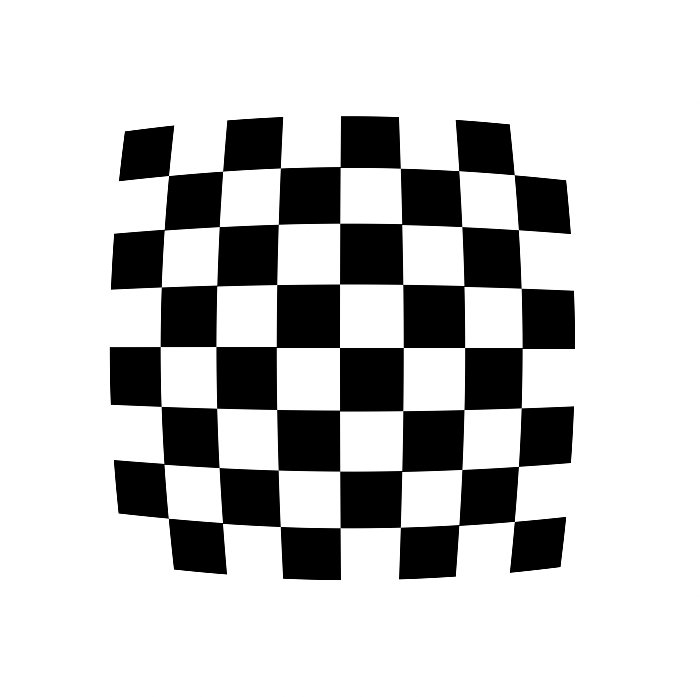
\includegraphics[trim = -2mm -2mm -2mm -2mm, width=0.3\textwidth]{figures/chess_input_3} }
  \subfloat[Corrected barrel-distorted image] { \label{fig:chess-3-o} 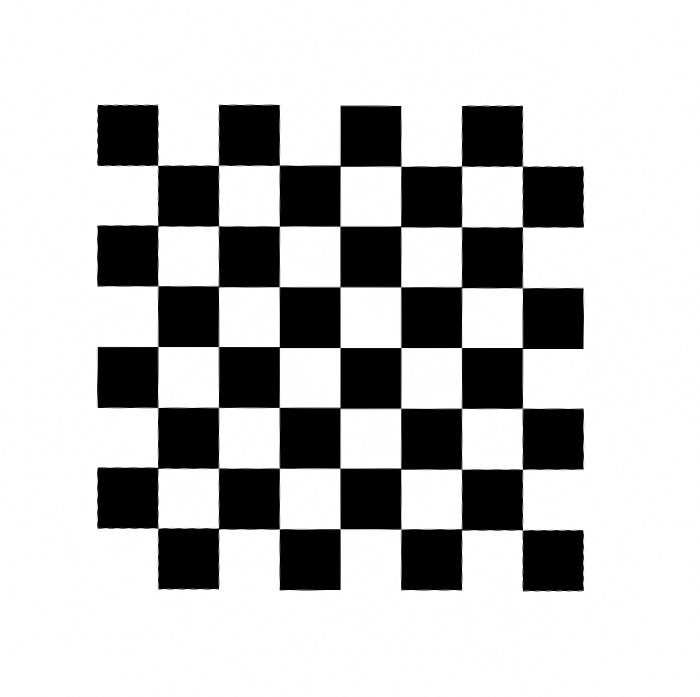
\includegraphics[trim = -2mm -2mm -2mm -2mm, width=0.3\textwidth]{figures/chess_output_3} }\\
  \subfloat[Pincushion-distorted image] { \label{fig:chess-4-i} 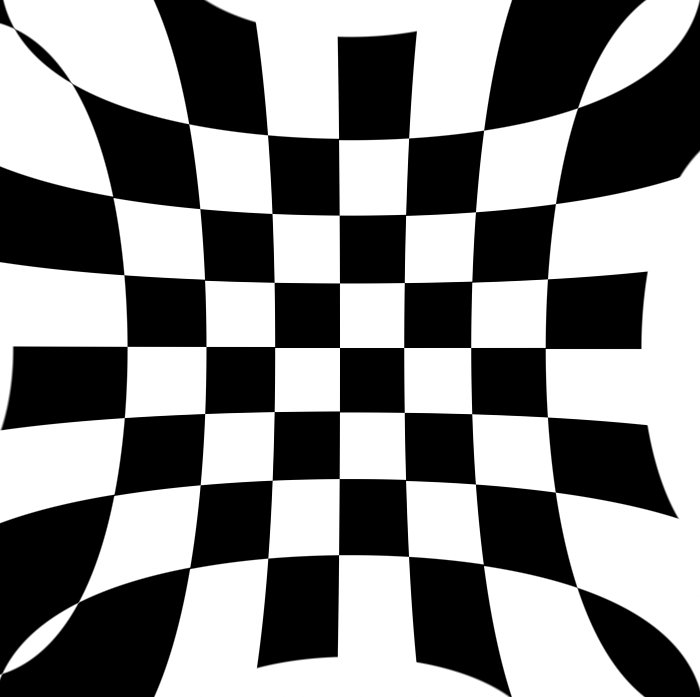
\includegraphics[trim = -2mm -2mm -2mm -2mm, width=0.3\textwidth]{figures/chess_input_4} }
  \subfloat[Corrected pincushion-distorted image] { \label{fig:chess-4-o} 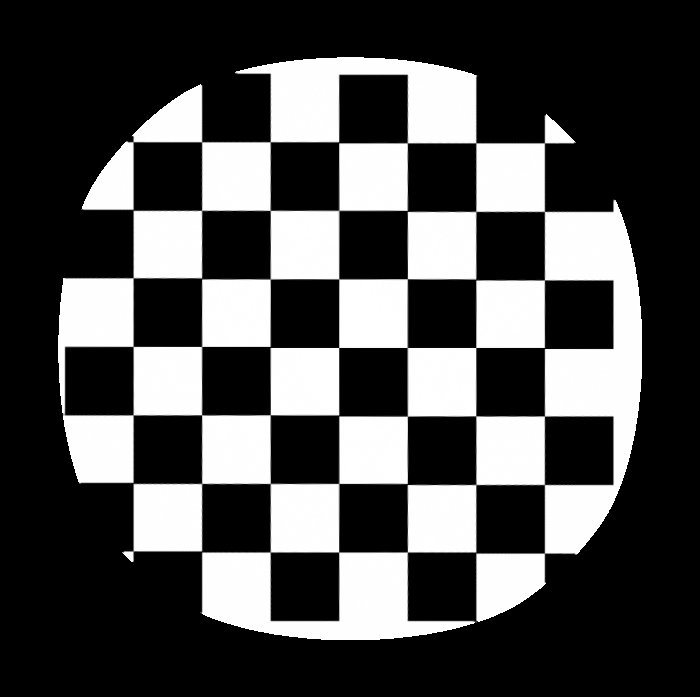
\includegraphics[trim = -2mm -2mm -2mm -2mm, width=0.3\textwidth]{figures/chess_output_4} }
  \caption{Chessboard images \#3 and \#4: barrel and pincushion distortion.}
  \label{fig:chess-3-4}
\end{figure}
  \item \textbf{A version with $90\%$ pincushion distortion likewise applied using GIMP.} Our program was only able to find 47 corners. Using straight lines based on these 47 points allowed the program to correct the image, but not perfectly: the chessboard corners remained distorted. See figure~\ref{fig:chess-4-o}. The algorithm found the following distortion model:\\
   $ \kappa_{0}$ : $1.071119593409116$\\
   $ \kappa_{2}$ : $-1.977158205506767 \times 10^{-006}$\\
   $ \kappa_{4}$ : $1.188341242264043 \times 10^{-014}$\\
   Note that all the $\kappa$ values have deviated in the opposite direction from their starting value than in the results for the barrel distortion image.
  \item \textbf{A standard chessboard tilted $22.5^o$.} The output was unchanged, as expected.
  \item \textbf{A standard chessboard tilted $45^o$.} The output was again unchanged.
  \item \textbf{A chessboard with barrel distortion, tilted $45^o$.} The output image appeared perfectly corrected. The lens distortion model found by the algorithm is extremely similar (to the second decimal place).
  \item \textbf{A chessboard with pincushion distortion, tilted $45^o$.} The algorithm was able to find all corners. However, the corrected image had the corners of its chessboard rounded, and some minor noise was added (see figure~\ref{fig:chess-8}). The algorithm found the following distortion model:\\
   $ \kappa_{0}$ : $1.032806607967469$\\
   $ \kappa_{2}$ : $-7.264872008702564 \times 10^{-007}$\\
   $ \kappa_{4}$ : $-3.242474093224431 \times 10^{-012}$\\
   This model is not quite as similar to the non-tilted pincushion-distorted image as its barrel-distorted analogue is to its own non-tilted version. This may be because pincushion distortion stretches the chessboard pattern over a greater relative area of the image, magnifying the effects of rotation at most points.
\begin{figure}[h]
  \centering
  \subfloat[Input image]{ \label{fig:chess-8-i} 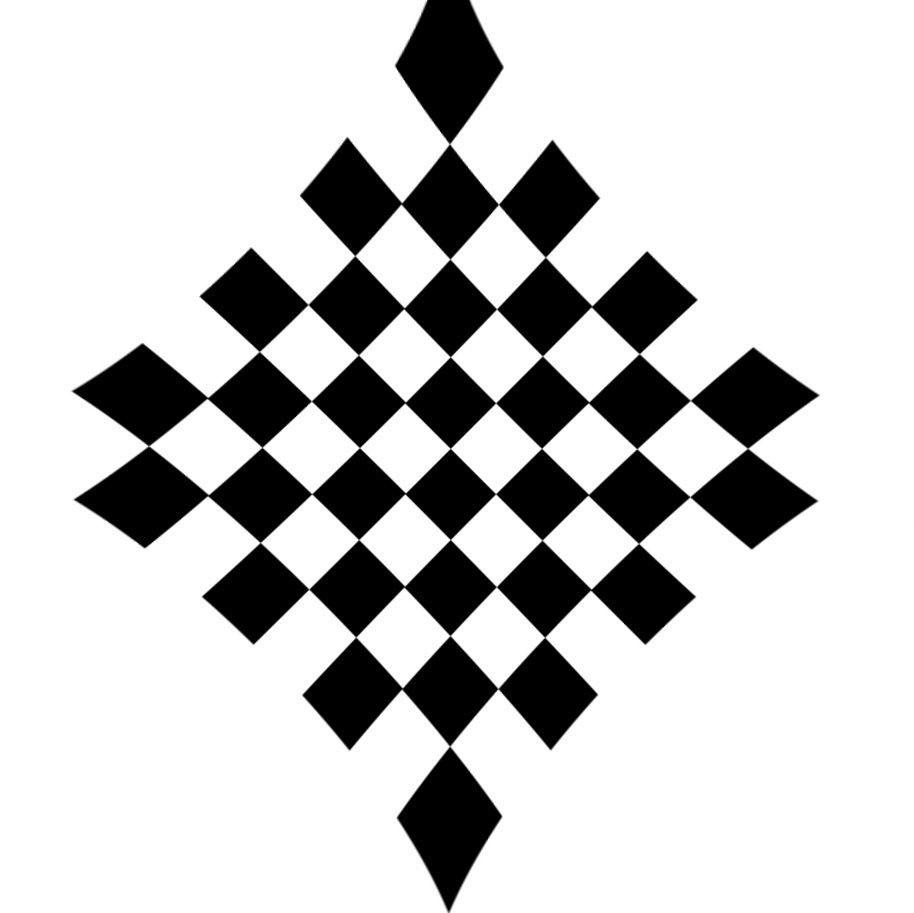
\includegraphics[trim = -2mm -2mm -2mm -2mm, width=0.3\textwidth]{figures/chess_input_8} }
  \subfloat[Output image]{ \label{fig:chess-8-o} 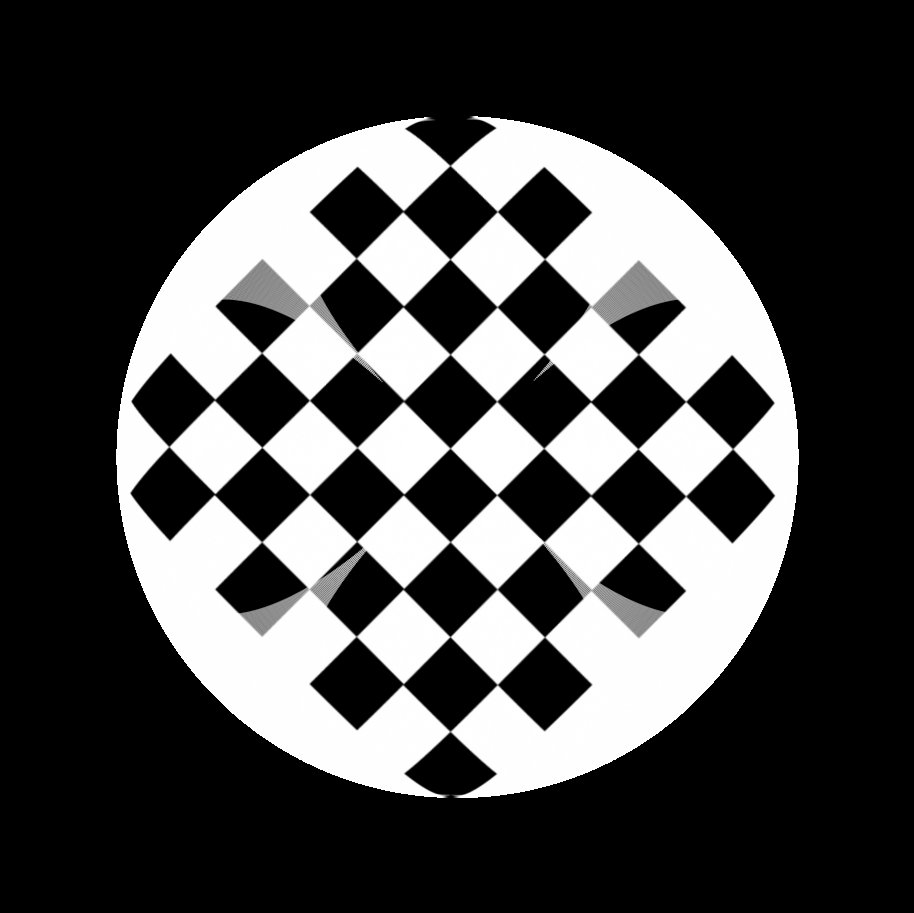
\includegraphics[trim = -2mm -2mm -2mm -2mm, width=0.3\textwidth]{figures/chess_output_8} }
  \caption{Chessboard image \#8: rotated pincushion distortion.}
  \label{fig:chess-8}
\end{figure}
  \item \textbf{A chessboard with barrel distortion, tilted $22.5^o$.} This was essentially the same as for the $45^o$ case. Again, the distortion model found by the algorithm was very similar to that for the un-tilted and more-tilted versions.
  \item \textbf{A chessboard with pincushion distortion, tilted $22.5^o$.} This was essentially the same as for the $45^o$ case. Once more, the distortion model found by the algorithm was very similar to that for the un-tilted and more-tilted versions.
  \item \textbf{A chessboard with barrel distortion, shifted within a larger image so that the centre of the board was not near the image centre.} This image was not properly corrected. In \cite{algebraic-distortion}, it is stated that the algorithm assumes the centre of the image is the distortion center: hence the failure of the algorithm on this irregular input. The program gives the following distortion model:\\
   $ \kappa_{0}$ : $1.025584574469791$\\
   $ \kappa_{2}$ : $-1.109909378582727 \times 10^{-006}$\\
   $ \kappa_{4}$ : $6.822970734639966 \times 10^{-012}$\\
   Interestingly, the values $\kappa_{0} > 1$, $\kappa_{2}$ < 0, $\kappa_{4}$ > 0 have strongly correlated with \emph{pincushion} distortion on other images.
  \item \textbf{A chessboard with pincushion distortion, similarly shifted within a larger image.} The algorithm could only find 47 corners in the image, and was unable to generate lines from these.
  \item \textbf{A barrel-distorted chessboard with a 10-pixel-wide Gaussian filter applied in GIMP.} The program was unable to detect any corner points with which to extract straight lines.
  \item \textbf{A pincushion-distorted chessboard with the same Gaussian filter.} The program was able to identify 37 of the corner points, but was again unable to extract straight lines using these.
  \item \textbf{A pincushion-distorted chessboard with noise added as the ``spread" function in GIMP (set to $10\%$).} The program only found 42 corners. For the first and only time in testing, it continued with applying IPOLdistortion functions to the invalid lines. These incorrect lines resulted in the strange pattern visible in figure~\ref{fig:chess-15-o1}. The distortion model returned was as follows:\\
   $ \kappa_{0}$ : $2.196137397890600$\\
   $ \kappa_{2}$ : $-9.717713325573065 \times 10^{-005}$\\
   $ \kappa_{4}$ : $9.424873711854491 \times 10^{-010}$\\
Note the unprecedentedly large value for $\kappa_{0}$. When the corners were reduced to 36 by the experimenter, the program managed to extract proper line segments, and apply distortion removal correctly. The output image for this had the corners of its chessboard lost (as in previous cases for pincushion distortion) but corrected the middle of the chessboard properly. See figure~\ref{fig:chess-15-o2}. The distortion model generated, which is much closer to the case for the baseline pincushion-distorted chessboard image, was:\\
   $ \kappa_{0}$ : $1.026807247150139$\\
   $ \kappa_{2}$ : $-1.318339975621756 \times 10^{-006}$\\
   $ \kappa_{4}$ : $-7.024131328406179 \times 10^{-012}$
\begin{figure}[h]
  \centering
  \subfloat[Input image]{ \label{fig:chess-15-i} 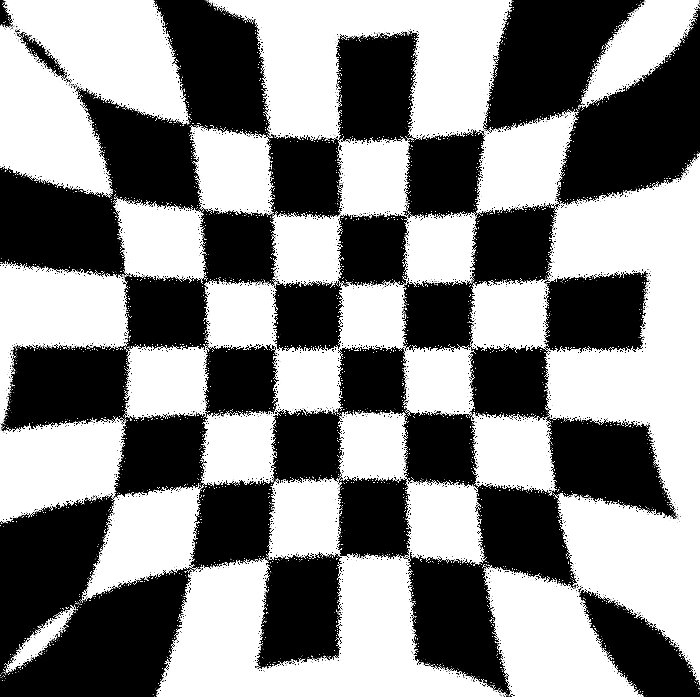
\includegraphics[trim = -2mm -2mm -2mm -2mm, width=0.26\textwidth]{figures/chess_input_15} }
  \subfloat[First output image]{ \label{fig:chess-15-o1} 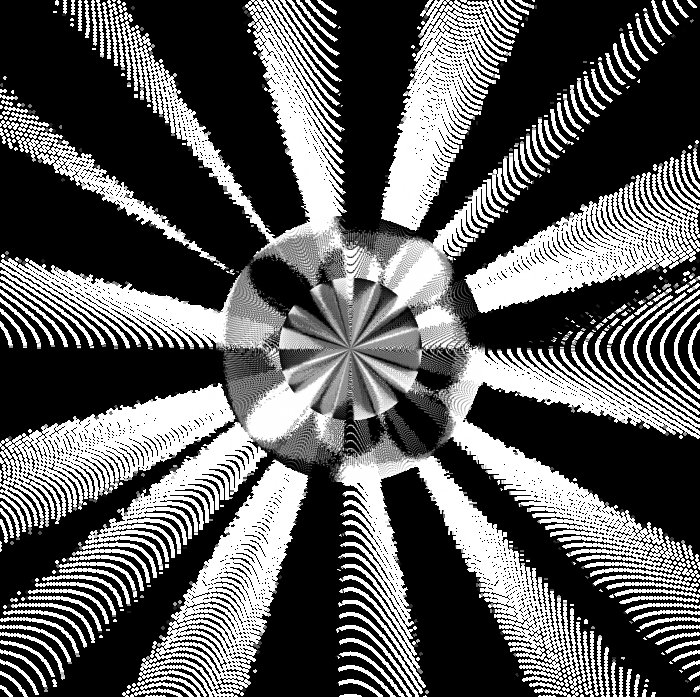
\includegraphics[trim = -2mm -2mm -2mm -2mm, width=0.26\textwidth]{figures/chess_output_15a} }
  \subfloat[Second output image]{ \label{fig:chess-15-o2} 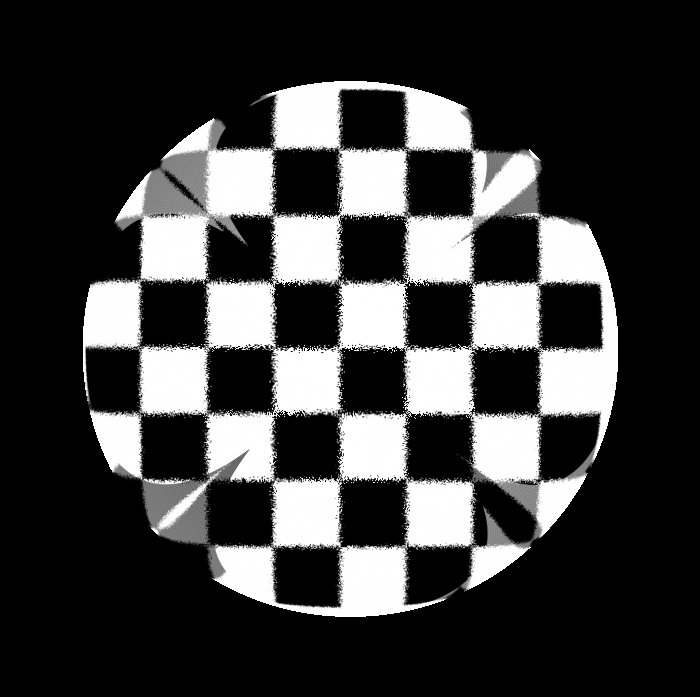
\includegraphics[trim = -2mm -2mm -2mm -2mm, width=0.26\textwidth]{figures/chess_output_15b} }
  \caption{Chessboard image \#15: pincushion distortion with $10\%$ spread noise.}
  \label{fig:chess-15}
\end{figure}
  \item \textbf{A similar pincushion-distorted chessboard, this time with $20\%$ noise.} The program was unable to detect any corner points with which to extract straight lines.
  \item \textbf{A barrel-distorted chessboard, with $10\%$ ``spread" noise.} The output image appeared perfectly corrected. The algorithm found the following distortion model:\\
   $ \kappa_{0}$ : $0.9536020990600429$\\
   $ \kappa_{2}$ : $1.548196267634160 \times 10^{-006}$\\
   $ \kappa_{4}$ : $1.618813812151320 \times 10^{-012}$\\
   The fact that the first two $\kappa$ coefficients are very similar (within the same order of magnitude) to those found for the baseline barrel-distorted chessboard image, on which this noisy image was based, suggests the algorithm is fairly robust.
  \item \textbf{A similar barrel-distorted chessboard, this time with $20\%$ noise.} The program could only find 28 of the chessboard corners, and was unable to extract lines from the image based on these.
  \item \textbf{A barrel-distorted chessboard with one edge of the board ``stretched" unevenly towards the image edge.} The program found all corners correctly, but the supposedly corrected image appeared almost unchanged from its original state; see figure~\ref{fig:chess-19}. This confirms that the IPOLdistortion algorithm is not equipped to model non-radial forms of distortion. The algorithm found the following distortion model:\\
   $ \kappa_{0}$ : $1.026810332882990$\\
   $ \kappa_{2}$ : $-9.847350544109156 \times 10^{-007}$\\
   $ \kappa_{4}$ : $4.754725445596508 \times 10^{-012}$\\
  As with the case for a barrel-distorted image of a non-central chessboard, we have values $\kappa_{0} > 1$, $\kappa_{2}$ < 0, $\kappa_{4}$ > 0, which otherwise correlate with \emph{pincushion} distortion.
\begin{figure}[h]
  \centering
  \subfloat[Input image]{ \label{fig:chess-19-i} 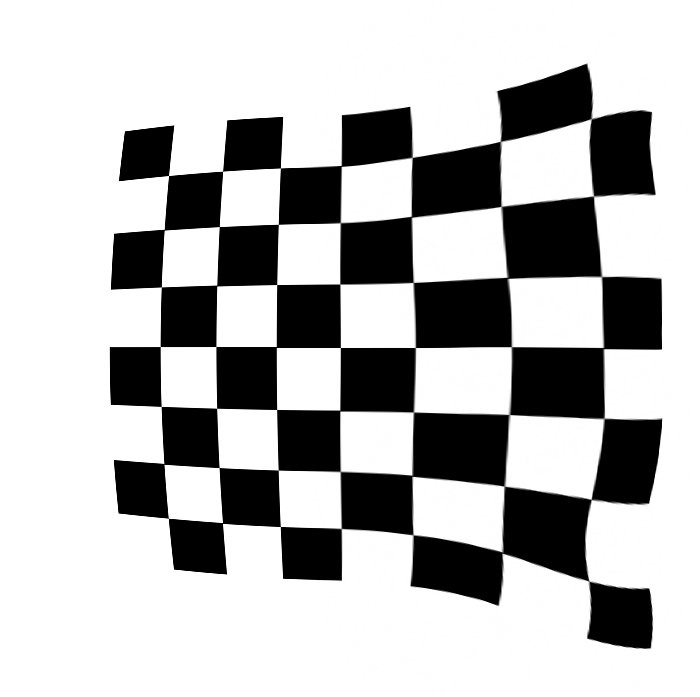
\includegraphics[trim = -2mm -2mm -2mm -2mm, width=0.3\textwidth]{figures/chess_input_19} }
  \subfloat[Output image]{ \label{fig:chess-19-o} 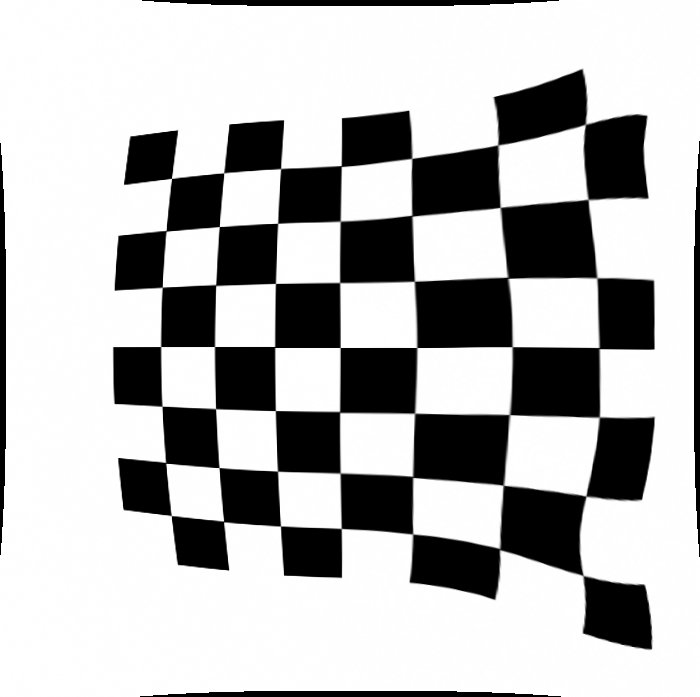
\includegraphics[trim = -2mm -2mm -2mm -2mm, width=0.3\textwidth]{figures/chess_output_19} }
  \caption{Chessboard image \#19: barrel distortion with stretched edge.}
  \label{fig:chess-19}
\end{figure}
  \item \textbf{A pincushion-distorted chessboard, with one edge stretched.} The program could find 27 to 33 corners in the middle (depending on the user's specification of the chessboard dimensionality), but was unable to extract line segments from the image.
  \item \textbf{A chessboard with one of its quadrants distorted by a function similar, but not identical, to pincushion distortion.} The program found all corners correctly, but the supposedly corrected image was at least as distorted as its original state (see figure~\ref{fig:chess-21}). Again, the algorithm clearly cannot correct non-radial distortion. The distortion model returned by the algorithm was very similar in $\kappa$ signs and magnitude to that for the ``stretched edge" and ``non central" barrel-distorted chessboards, which it also failed to model.
\begin{figure}[h]
  \centering
  \subfloat[Input image]{ \label{fig:chess-21-i} 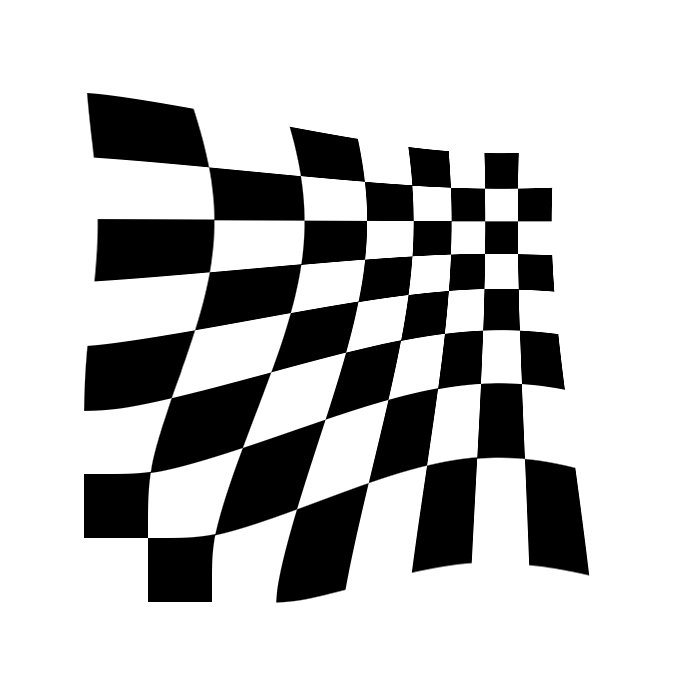
\includegraphics[trim = -2mm -2mm -2mm -2mm, width=0.3\textwidth]{figures/chess_input_21} }
  \subfloat[Output image]{ \label{fig:chess-21-o} 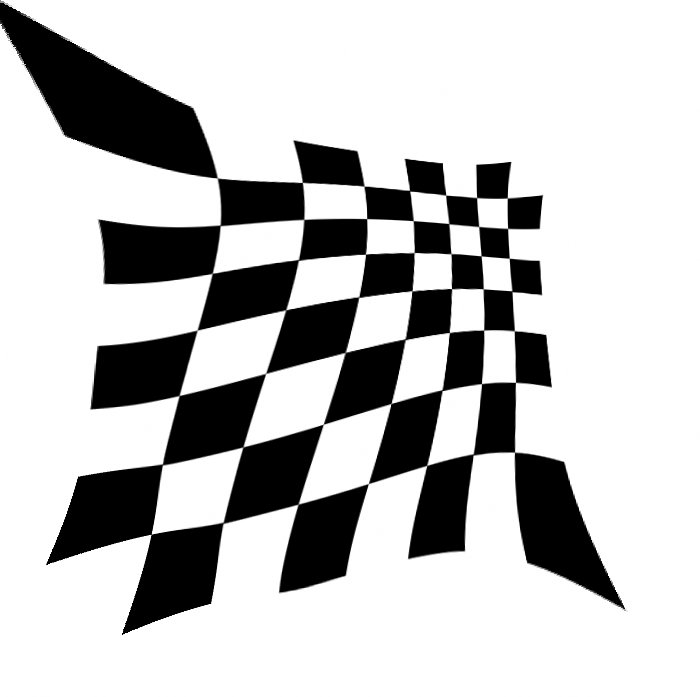
\includegraphics[trim = -2mm -2mm -2mm -2mm, width=0.3\textwidth]{figures/chess_output_21} }
  \caption{Chessboard image \#21: pseudo-pincushion distortion in one chessboard quadrant.}
  \label{fig:chess-21}
\end{figure}
  \item \textbf{A chessboard with one of its quadrants distorted this time by a function similar, but not identical, to barrel distortion.} The program could find 47 of the corners, but was unable to extract lines from the image.
\end{enumerate}

\paragraph{Other tests.}
We also ran our program on a wide range of pseudo-chessboard images obtained in various ways: from internet searches, created by hand from distorted grids drawn by hand, or created by hand from distorted grids acquired from internet searches. These tests confirmed our results from running the program on our artificial chessboard suite. We determined that images of chessboards of strange dimensionalities (such as 4x10 or 14x16) can be corrected, assuming reasonable sizes for the chessboard squares. We noted that the algorithm often cannot handle extreme camera angles or unusual types of noise (such as ``ink blotch" style noise, or significant noise at the corner-points of chessboard squares).

\subsubsection{Comparison with camera calibration results}

The process of camera calibration also involves determining the lens distortion parameters of the camera used to create an image. We tested our results with Tsai calibration from section~\ref{sec:calibration}. We took an image of the distortion object, and the images of its artificially barrel-distorted and pincushion-distorted variants, and generated lists of line segments for each. These lines were created from the image calibration points, which ought to lie on straight lines on each face. For each of the three images, we used all horizontal lines on each face as well as the two outer vertical lines from each face, for a total of 18 lines per image. We ran the code from the IPOLdistortion library directly on these lines, and compared the $\kappa_{0}$, $\kappa_{2}$, and $\kappa_{4}$ coefficients that were generated to the $\kappa_{1}$ found by Tsai calibration.

\begin{table}[htb]
  \centering
  \begin{tabular}{| l | c c c | c |}
    \hline
    {\textbf{ }} &
    {\textbf{$\kappa_{0}$ (IPOL)}} &
    {\textbf{$\kappa_{2}$ (IPOL)}} &
    {\textbf{$\kappa_{4}$ (IPOL)}} &
    {\textbf{$\kappa_{1}$ (Tsai)}}\\
    \hline
    {\textbf{Normal}} & { } & { } & { } & { } \\
    {\textbf{calibration}} & {$1.0063$} & {$-2.746 \times 10^{-08}$} & {$1.926 \times 10^{-14}$} & {$-1.513 \times 10^{-08}$} \\
    {\textbf{image}} & { } & { } & { } & { } \\
    \hline
    {\textbf{Barrel}} & { } & { } & { } & { } \\
    {\textbf{-distorted}} & {$0.9659$} & {$9.536 \times 10^{-08}$} & {$3.814 \times 10^{-14}$} & {$1.194 \times 10^{-07}$} \\
    {\textbf{image}} & { } & { } & { } & { } \\
    \hline
    {\textbf{Pincushion}} & { } & { } & { } & { } \\
    {\textbf{-distorted}} & {$1.0583$} & {$-1.389 \times 10^{-07}$} & {$-6.806 \times 10^{-15}$} & {$-1.731 \times 10^{-06}$} \\
    {\textbf{image}} & { } & { } & { } & { } \\
    \hline
  \end{tabular}
  \caption[Comparison of Tsai calibration and IPOLdistortion lens distortion models]{Comparison of Tsai calibration and IPOLdistortion lens distortion models. The first three columns give the $\kappa_{0}$, $\kappa_{2}$, and $\kappa_{4}$ coefficients determined by the distortion removal code. The fourth column gives the $\kappa_{1}$ coefficient found by Tsai calibration.}
  \label{tbl:calib-distort-compare}
\end{table}

The results are presented in table~\ref{tbl:calib-distort-compare}. The distortion models are not immediately comparable, obviously, because the mathematical model developed by \cite{algebraic-distortion} ranges over even $\kappa$ values, whereas our implementation of Tsai calibration only calculates $\kappa_{1}$.

However, we observe that both forms of distortion modelling have the lowest $\kappa$ coefficients when run on the normal image; distortion increases for the barrel-distorted image, and increases significantly more (by as much as an order of magnitude) for the pincushion-distorted image. For all three image variants, the $\kappa_{1}$ calculated in Tsai calibration is closest to the $\kappa_{2}$ of IPOLdistortion - in magnitude and in sign. This is expected, given that both these $\kappa$ values are calculated by optimisation from the value $0$, whereas $\kappa_{0}$ (which might otherwise be considered equally close to $\kappa_{1}$) is calculated in the IPOLdistortion algorithm by optimisation from the value $1$.

The results of the two algorithms appear similar. Although we lack the testing apparatus to say so definitively, it is almost certain that the IPOLdistortion is the better distortion modeller and corrector (within the bounds of a typical lens distortion system). We say so because of our qualitative confirmation of the success of the IPOLdistortion algorithm on suitable test images, and the simplistic (single $\kappa$) nature of the distortion model calculated as part of our Tsai calibration.
